\chapter{Seismic Noise}
Seismic noise causes two issues for laser interferometric gravitational-wave detectors; (1) limitation of the low-frequency sensitivity of the detectors and (2) deterioration of the duty cycle of that. The former problem caused by the seismic noise above $1\,\mathrm{Hz}$, which is associated with anthropogenic activity. On the other hand, the latter problem caused by the seismic motion below this frequency, which is generated by the natural noise source such as the ocean, disturbe the Fabry-Perot arm cavity to resonate stably.

In order to resolve these issues, a laser interferometer gravitational wave antenna with a baseline length of 20 m (LISM) \cite{sato2004ultrastable} is constructed underground, because the low-level seismic noise is expected in the undeground environment. As a result, the seismic noise in LISM site is less than that in the surface site by two prders of magnitude in $1$--$100\mathrm{Hz}$ region, and the underground GW detector performanced stable operation with duty cycle of $99.8 \%$.

However, for km-meter scale GW detector like KAGRA, such a stable operation can not be expected because
\begin{itemize}
  \setlength{\itemsep}{1pt}      %2. ブロック間の余白
  \setlength{\parskip}{-1pt}     %4. 段落間余白.
  \setlength{\itemindent}{0pt}   %5. 最初のインデント
  \setlength{\labelsep}{5pt}     %6. item と文字の間
\item length of the long baseline is susceptible to the low-frequency seismic motion compared with the short one due to the a few reduction effect kind of the {\it common mode rejection}, and this problem is common in not only all the current detectors but also the next $10\,\mathrm{km}$-scale detectors; Einstein Telescope (ET)\cite{punturo2010einstein} and Cosmic Exploler (CE) \cite{abbott2017exploring}.
\item especially in KAGRA site, the microseismic noise corelated with the ocean activity in $0.03$--$0.3\,\mathrm{Hz}$, which is the most problematic noise for stable operation of GW detector, cannot be reduced even in the underground due to near the sea ($40\,\mathrm{km}$ from Toyama Bay), and this problem is common in ET which is also will be constructed in underground but in island \cite{naticchioni2014microseismic}.
\end{itemize}
The purpose of this chapter is to describe quantitatively above two problems. In this chapter, first, section \cref{sec:31} gives an theoretical understanding of the seismic noise as the elastic waves. In section \cref{sec:32}, some general properties of the seismic noise are described by quotting previous researches. Finally, we discuss the problems in section \cref{sec:33}.



\section{Theory of seismic waves} \label{sec:31}
Here we introduce characteristics of the seismic wave that will be usefull in our later understanding and modeling of seismic effects.



\subsection{Seismic Waves}
The elastrodynamic wave equation without external forces is given by 
\begin{eqnarray}\label{eq:eq_1}
  \rho{\bm{\ddot{u}}} = (\lambda+2\mu)\nabla(\nabla\cdot\bm{u}) - \mu\nabla\times(\nabla\times\bm{u}),
\end{eqnarray}
where $\bm{u}$ is the displacement field vetor of the medium, $\rho$ denotes density of the medium, and $\lambda,\,\mu$ are Lame's first and second parameter.



\subsubsection{Body Waves}
From Eq.(\ref{eq:eq_1}), we can obtain two characteristic waves; longitudinal wave (primary wave, P-wave) and transverse wave (secondary wave, S-wave). First, using Helmholtz's decomposition, we represent the displacement field vector $\bm{u}$ as
\begin{eqnarray} 
  \bm{u} &=& \nabla\phi + \nabla\times\bm{\psi}, \label{eq:eq_4}
\end{eqnarray}
where $\phi$ the scalar potential and $\bm{\psi}$ are the vector potential. Each term of Eq.(\ref{eq:eq_4}) show the divergent and the rotation component of $\bm{u}$ respectively. Substitute Eq.(\ref{eq:eq_4}) into Eq.(\ref{eq:eq_1}) and after some vector algebra, one can obtain two wave equations;
\begin{eqnarray}
  \ddot{\phi} &=& v_{L}^2\nabla^2\phi \label{eq:eq_5},\\
  \ddot{\psi} &=& v_{T}^2\nabla^2\psi \label{eq:eq_6}, 
\end{eqnarray}
where $v_{L},\,v_{T}$ are defined as 
\begin{eqnarray}
  v_{L} = \sqrt{\frac{\lambda+2\mu}{\rho}},\
  v_{T} = \sqrt{\frac{\mu}{\rho}}. \label{eq:eq_7}
\end{eqnarray} 
These phase velocities; $v_{L},v_{T}$ represent that of the P-wave and the S-wave. Show this relationships. Because the scalar potential and the vector potential are obey the wave equation Eq.(\ref{eq:eq_5}) and Eq.(\ref{eq:eq_6}) respectivly, the general solutions of these potentials are given as
\begin{eqnarray}
  \phi &=& \phi_{0}(\omega{t}-\bm{k}\cdot{\bm{x}}) \label{eq:eq_8}\\
  \bm{\psi} &=& \bm{\psi_{0}}(\omega{t}-\bm{k}\cdot{\bm{x}}) \label{eq:eq_9},
\end{eqnarray}
where $\omega,\,\bm{k}$ are the angler frequency and the wave vector. One can obtain the divergent component of displacement filed vector $\bm{u}$ as
\begin{eqnarray}
  \bm{u}_{\mathrm{div}} = \nabla{\phi_{0}(\omega{t}-\bm{k}\cdot{\bm{x}})} =-\bm{k}{\phi}.
\end{eqnarray}
The displacement of this wave $\bm{u}_{\mathrm{div}}$ whose phase velocity is $v_{L}$ propagates along with direction of the wave vector. Therefore $v_{L}$ is the phase velocity of a longitudinal wave called P-wave. On the other hands, one can obtain the rotation component of $\bm{u}$ as
\begin{eqnarray}
  \bm{u}_{\mathrm{rot}} = \nabla\times{\bm{\psi_{0}}(\omega{t}-\bm{k}\cdot{\bm{x}})} =-\bm{k}\times{\bm{\psi}}.
\end{eqnarray}
This displacement vector $\bm{u}_{\mathrm{rot}}$ whose phase velocity is $v_{T}$ is perpendicular to the wave vector. Therefore, $v_{T}$ is the phase velocity of a transverse wave called S-wave. Furthermore, because  $\lambda$ and $\mu$ are positive numbers, 
\begin{eqnarray}
  v_{L} > v_{T}.\label{eq:eq_10}
\end{eqnarray}
Therefore, the longituginal wave is faster than the transverse wave.



\subsubsection{Rayleigh waves}
Rayleigh wave is produced by the interfer of P-wave and S-Wave \cite{hasegawa2015jishin}. \textcolor{red}{ここではZ軸を鉛直方向とした直交直線座標系のx-z面内で振動する弾性波を考える。z=0を自由表面とし、x軸に沿ってP波とS波が同じ速度$v_{R}=\omega/k$ ($\omega$ is anglar frequency and $k$ is the wave vector) で伝搬する場合を考えると、ポテンシャル$\phi$と$\bm{\psi}$は、それぞれ以下のように表すことができる。
\begin{eqnarray}
  \phi &=& F(z)\exp[i(kx-\omega{t})],\label{eq:eq_12}\\
  \psi &=& G(z)\exp[i(kx-\omega{t})]\label{eq:eq_13}
\end{eqnarray}
Eq.\ref{eq:eq_12}とEq.\ref{eq:eq_12}を波動方程式Eq.\ref{eq:eq_5},Eq.\ref{eq:eq_6}に代入すれば、レイリー波の特性方程式が導かれる;
\begin{eqnarray}\label{eq:eq_11}
\left(\frac{c_{R}^{2}}{c_{S}^{2}}\right)^{3}-8\left(\frac{c_{R}^{2}}{c_{S}^{2}}\right)^{2}+8\left(3-\frac{2}{\gamma^2}\right)\left(\frac{c_{R}^{2}}{c_{S}^{2}}\right)-16\left(1-\frac{1}{\gamma^2}\right)=0
\end{eqnarray}
where $\gamma\equiv v_{L}/v_{T}$. In case that $0 < (\frac{c_{R}^2}{c_{S}^2}) <1$, the velocity has physically meaningful value. According to Eq.\ref{eq:eq_11}, the ratio $\frac{c_R}{c_S}$ is a function of the ratio of $\gamma$. たとえば、KAGRAと同じ山の下に建設された100mの重力波望遠鏡CLIOでのP波とS波の位相速度はそれぞれAA、BBである\cite{takemoto2003}ので、$\gamma = 1.82 $である。したがってこのときのレイリー波の位相速度はCCである。
}



%% \subsection{Reduction Effect in the Deep Sites}
%% \textcolor{red}{
%%   レイリー波の振幅は深さに依存しており、深いほど小さくなる。
%% }



\subsection{Reduction Effect of the Short Baseline} \label{sec:313}
For interferometric gravitational-wave detectors which need a precise length control of the optical resonate cavity, it is appropriate to consider about the relative displacement between two points rather than the displacement of single point.



\subsubsection{Differential Motion and Common Motion}
We define the motion of two points shown in Fig.(\ref{img:img310}) as $\bm{u}_1=\bm{u}(t,\bm{x}_1)$ and $\bm{u}_2=\bm{u}(t,\bm{x}_2)$, respectively. The motions of the two points can be represented as the differential motion and the common motion. The displacement of both differential motion and common motion of the two points shown in Fig.(\ref{img:img310}) are defined as
\begin{eqnarray}
  \bm{u}_{\mathrm{diff}} \equiv \frac{\bm{u}_{1}-\bm{u}_{2}}{\sqrt{2}}, \, \\ \label{eq:eq22}
  \bm{u}_{\mathrm{comm}}  \equiv \frac{\bm{u}_{1}+\bm{u}_{2}}{\sqrt{2}} \label{eq:eq100}
\end{eqnarray}
These two motions defined in Eq.(\ref{eq:eq22}) and Eq.(\ref{eq:eq100}) are normalized by $\sqrt{2}$ to conserve the total power.
\begin{figure}[h]
  \begin{center}
    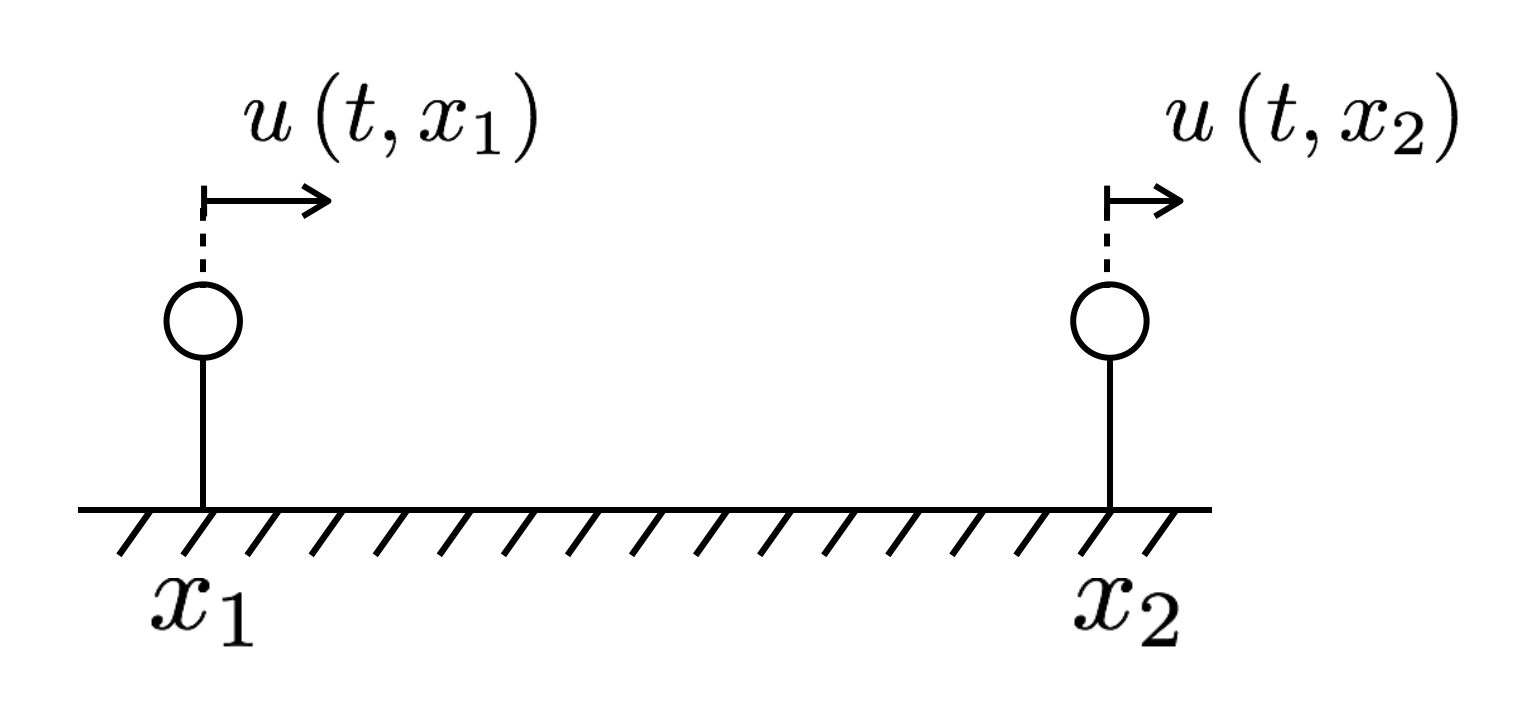
\includegraphics[width=9.0cm]{./img_chap3/img315.png}
    \caption{The displacements of the two points which are sparated L in X axis. $\bm{u}(t,\bm{x})$ is the displacement field vector, where $t$ denotes the time and $\bm{x}$ denotes the location vector.}\label{img:img310}    
  \end{center}
\end{figure}



\subsubsection{Common and Differential Motion Ratio (CDMR)}\label{sec:sec313}
We define the power ratio of the common motion over the differential motion as common and differential motion ratio (CDMR). This ratio is usefull to describe how the differential motion is reduced in the baseline compared to the common motion. CDMR is defined as
\begin{equation}
  \mathrm{CDMR} \equiv \sqrt{\frac{\mathrm{Common\,Motion}}{\mathrm{Differential\,Motion}}} = \sqrt{\frac{P_{\mathrm{comm}}(\omega)}{P_{\mathrm{diff}}(\omega)}} \label{eq:eq23}
\end{equation}
where $P_{\mathrm{comm}},P_{\mathrm{diff}}$ are the power spectral densities (PSDs) of the differential motion and common motion, respectively. In order to obtain these PSDs, we convert from the autocorrelation function of these. Therefore, first, autocorrelation function $C_{\mathrm{diff}}$ of the differential motion is given by its definition in Eq.(\ref{eq:eq22})
\begin{eqnarray}
  C_{\mathrm{diff}}(\tau) &=& \frac{1}{2}
  \biggl\langle
  \biggl[ x_{1}(t)-x_{2}(t) \biggr] \biggl[ x_{1}(t+\tau)-x_{2}(t+\tau) \biggr]
  \biggr\rangle \\
  &=& \frac{1}{2}\biggl[ C_{11}(\tau) - C_{12}(\tau) - C_{21}(\tau) + C_{22}(\tau) \biggr], 
\end{eqnarray}
,where $C_{ij}$ are the autocorrelation functions of each point and defined as $ C_{ij} \equiv \langle x_{i}(t)x_{j}(t+\tau)\rangle,\, (i=1,2,\,j=1,2)$. Here, one can obtain the power spectrum density of differential motion $P_{\mathrm{diff}}(\omega)$ as 
\begin{eqnarray}
  P_{\mathrm{diff}}(\omega) &=& \frac{1}{2}\biggl[ P_{1}(\omega) + P_{2}(\omega) - P_{12}(\omega) - P_{12}^*(\omega) \biggr]\\
  &=& \frac{1}{2} \biggl[ P_{1}+P_{2} - \mathrm{Re}\left[\gamma \right]\times2\sqrt{P_{1}P_{2}} \biggr], \label{eq:eq31}
\end{eqnarray}
where $P_{1}(\omega),P_{2}(\omega)$ are the power spectrum densities of each points, and $P_{12}(\omega)$ are the cross spectrum between two point. The parameter $\gamma$ is the complex coherence between them defined by
\begin{eqnarray}
  \gamma \equiv \frac{P_{12}}{\sqrt{P_{1}P_{2}}}.
\end{eqnarray}
Furthermore, assuming that seismic wave propagating each points does not decay, which means $P_{1}=P_{2} \equiv P$, one can compute the $P_{\mathrm{diff}}(\omega)$ as 
\begin{eqnarray} \label{eq:eq32}
  P_{\mathrm{diff}}(\omega) = P (1-\mathrm{Re}\left[\gamma\right]).
\end{eqnarray}
Similarly, the PSD of the common motion can be calculated as
\begin{eqnarray}
  P_{\mathrm{comm}}(\omega) = P (1+\mathrm{Re}\left[\gamma\right]).
\end{eqnarray}
Finaly, CDMR defined Eq.(\ref{eq:eq23}) in case the seismic wave does not decay is represented as
\begin{eqnarray}
 \mathrm{CDMR} = \sqrt{\frac{1 + \mathrm{Re} \left[\gamma \right] }{1 - \mathrm{Re} \left[\gamma \right]}}\,. \label{eq:eq33}
\end{eqnarray}
Eq.(\ref{eq:eq33}) indicates that CDMR can be expressed by only the coherence $\gamma$ between of two points. For example, CDMR tends to be larger when $\gamma$ close to 1. This means that the differential motion is more less than the common motion because the two points move together in the same direction.


\subsubsection{Uniform Plane Wave Model}
Consider the CDMR when the plane waves are distributed uniformly around the azimuth. Because the coherence in case that the single plane wave propagating with the azimuth angle $\theta$ along the direction of arm cavity from $x_1$ to $x_2$ in Fig.(\ref{img:img310}) is given by
\begin{equation}
  \gamma = \exp\left[{i\frac{L\mathrm{cos}\theta\omega}{c}}\right], \label{eq:eq18}
\end{equation} 
the coherence in case that the plane waves propagats uniformly is given by the integral of Eq.(\ref{eq:eq18}) over all direction;
\begin{eqnarray} \label{eq:eq19}
  \gamma &=& \frac{1}{2\pi} \int_{-\pi}^{\pi} e^{i\frac{\omega}{c} L\cos \theta} d \theta .
\end{eqnarray}
where the coherence is normized azimuth angle. Therefore, the CDMR is given as
\begin{equation}  \label{eq:eq20}
  \mathrm{CDMR} = \sqrt{\frac{1+J_0(\frac{L\omega}{c})}{1-J_0(\frac{L\omega}{c})}} .
\end{equation}

For later discussion in \cref{sec:332}, the PSD of the differential motion in case of the uniform seismic waves is usefull and is given as
\begin{eqnarray} \label{eq:eq21}
  P_{\mathrm{diff}}(\omega) = P \left[1-J_0\left(\frac{L\omega}{c}\right)\right] .
\end{eqnarray}

\subsubsection{Comparison with different baseline length}
The CDMR comparison with LISM, CLIO, KAGRA is shown in Fig.\ref{img:img301}. We assume that the uniform plane wave model with phase velocity of $3\,\mathrm{km/sec}$. One can find that km-scale detector has few CDMR below $0.1\,\mathrm{Hz}$ than the other short-scale detectors. 



\begin{figure}[p]
  \begin{center}
    \centering
    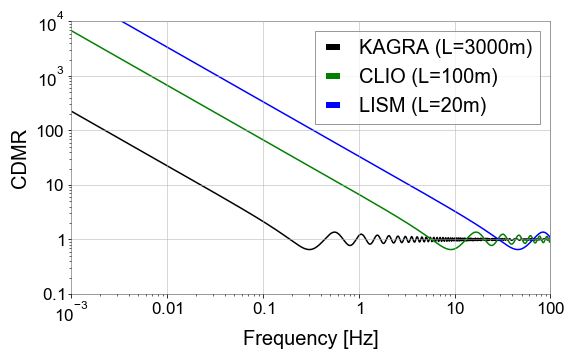
\includegraphics[width=12cm]{./img_chap3/img329.png}
    \caption{CDMR, which is the power ratio of the common motion over the differential motion of baseline in Eq.(\ref{eq:eq20}), of the underground GW detectors assuming the uniform plane waves model with phase velocity of 3000 m/sec. Black is KAGRA with the 3000 m baseline, green is CLIO with the 100 m baseline, and blue is LISM with the 20 m baseline. The CDMR of the long baseline is worse than that of short baseline.}\label{img:img301}
    \centering      
    %% 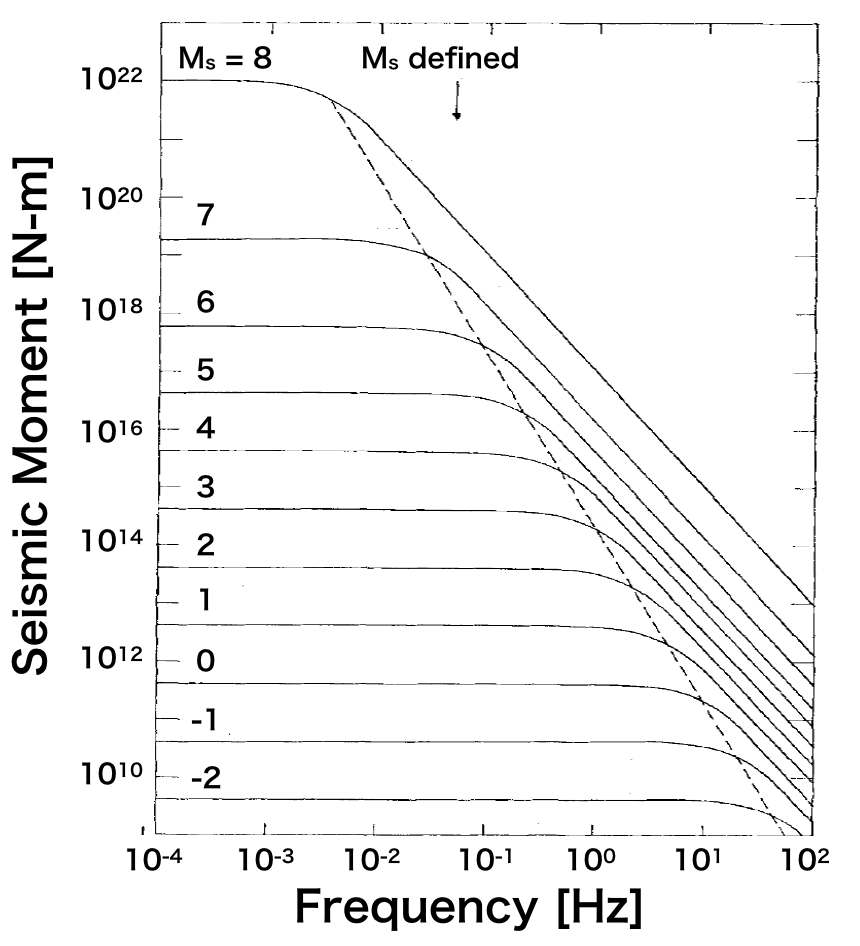
\includegraphics[width=12cm]{./img_chap3/img328.png}
    %% \caption[The power ratio of the differential motion of the baseline over the motion at single point; $P_{\mathrm{diff}}/P$ of Eq.(\ref{eq:eq21})]{The power ratio of the differential motion of the baseline over the motion at single point; $P_{\mathrm{diff}}/P$ of Eq.(\ref{eq:eq21}). This ratio gives the estimation of the PSD of baseline length fluctuation from the }\label{img:img302}
  \end{center}
\end{figure}


\newpage
\section{Seismic Noise}\label{sec:32}
Characteristics of the seismic noise are related with its origin spatially and temporally. The noise sources are spreaded anywhere; foot steps, traffics and ocean waves, and these amplitude depends on day-night or weather condition.

As summarized in Table \ref{tb:31}, the seismic noises above $1\,\mathrm{Hz}$ are cleary correlated with cultural activities, and that below this frequency are excited by the natural phenomena \cite{bonnefoy2006nature}.
\begin{table}[h] 
  \begin{center}
    \caption{Two types of seismic noise}\label{tb:31}
    \begin{tabular}{lll} 
      \hline      
      Type of noise & Frequency Band & Sources \\ \hline \hline
      Cultural Noise & $> 1\,\mathrm{Hz}$ & wind, traffic, machinaries, foot steps\\
      Natural Noise  & $< 1\,\mathrm{Hz}$ & ocean, air pressure, earth tides\\
    \end{tabular}
  \end{center}
\end{table}

This boundary frequency between cultural or natural is depends on the soil structure. At the sediment site such as the LIGO \cite{Daw_2004} and Virgo site \cite{Beker_2012}, the cultural noise can be shifted to a lower frequency and appear below $1\,\mathrm{Hz}$. On the other hands, at the hard rock site such as KAGRA site, the cultural noise can be distinguished from the natural noise for its diurnal variability and apparent only above $1\,\mathrm{Hz}$.


\subsection{Cultural Noises} \label{sec:321}
The cultural seismic noise contaminates the sensitivity of gravitational-wave detectors in the frequency range of interest for gravitational-waves sources, above $1\,\mathrm{Hz}$. In this frequency band, the cultural noise is dominated by winds or human activities. For example, seismic noise from traffic near the detectors is reported at LIGO site \cite{schofield2000source}, and noise from the vibrations of building excited by winds is reported at Virgo site \cite{acernese2004properties}. 

\subsection{Natural Noises} \label{sec:322}
The natural seismic noise affects the stability of the GW detectors below $1\,\mathrm{Hz}$ because it deforms the ground on which mounted the detectors.

These natural noises depends on the location. Fig.\ref{img:img324} shows the noise spectral of the seismic noise measured by Peterson in 75 stations in the world \cite{peterson1993observations}. The NHNM is a spectrum of average of high background noise power in the stations. Moreover the primary contributions to NHNM are coastal stations and inland stations on the soft soil. On the other hand, the NLNM represents the seismic noise when microseismic is quiet. Especially, below microseismic, it represents the global seismic noise floor \cite{nishida2002origin}. 

\begin{figure}[p]
  \begin{center}   
    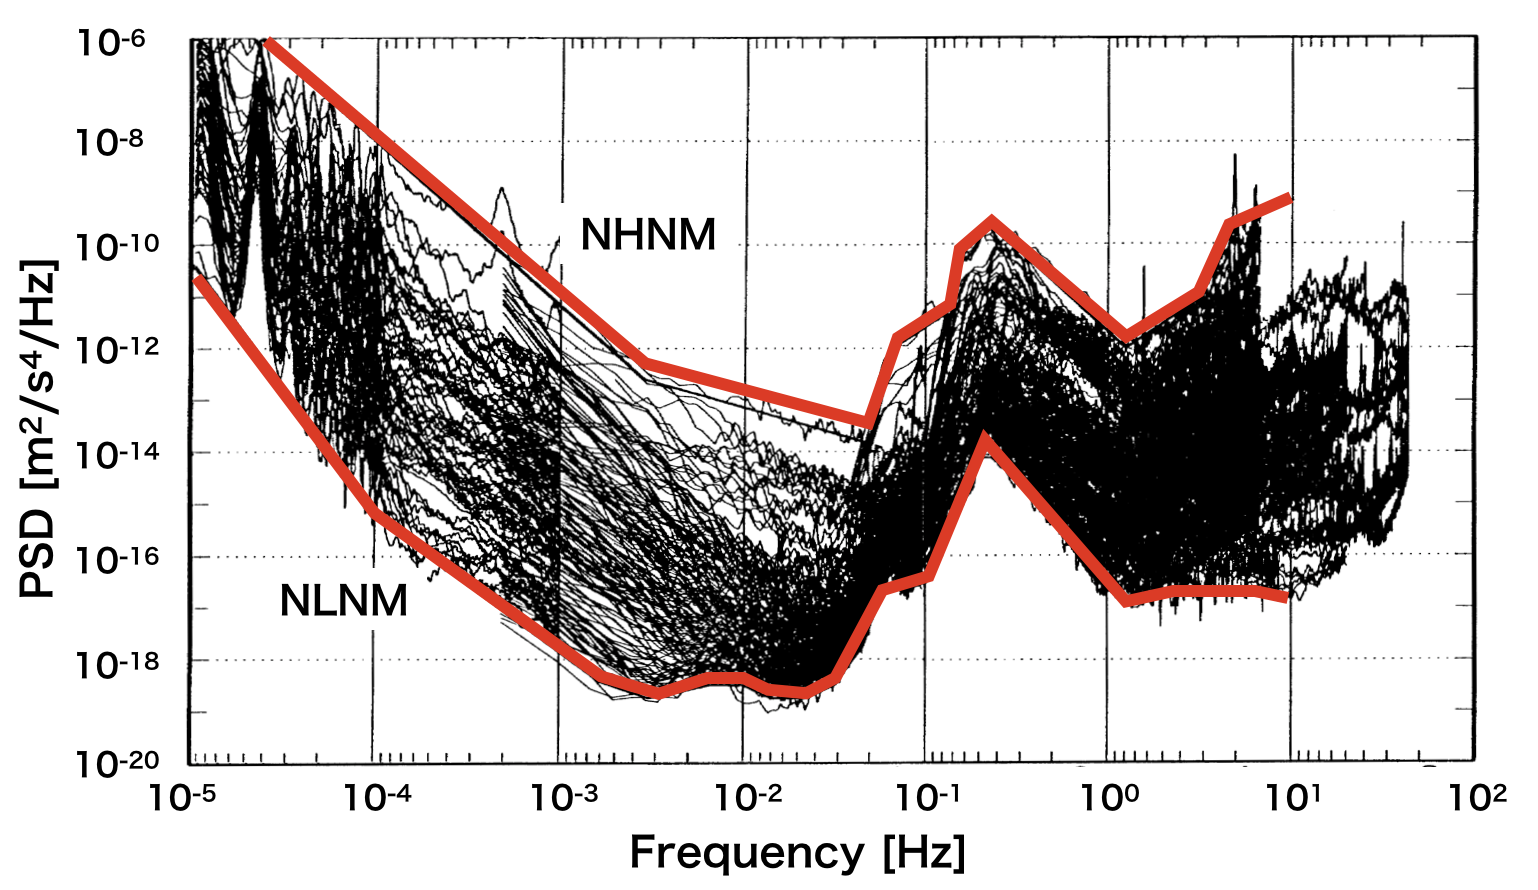
\includegraphics[width=12.5cm]{./img_chap3/img324.png}
    \caption{PSDs of the seismic noise obtained by Peterson in 75 stations in the world \cite{peterson1993observations}. Each of the black solid lines is PSD divided into 5 different frequency band at the each stations. Each red lines are the new high noise model (NHNM) and the new low noise model (NLNM), respectively.}\label{img:img324}
  \end{center}
  \begin{center}   
    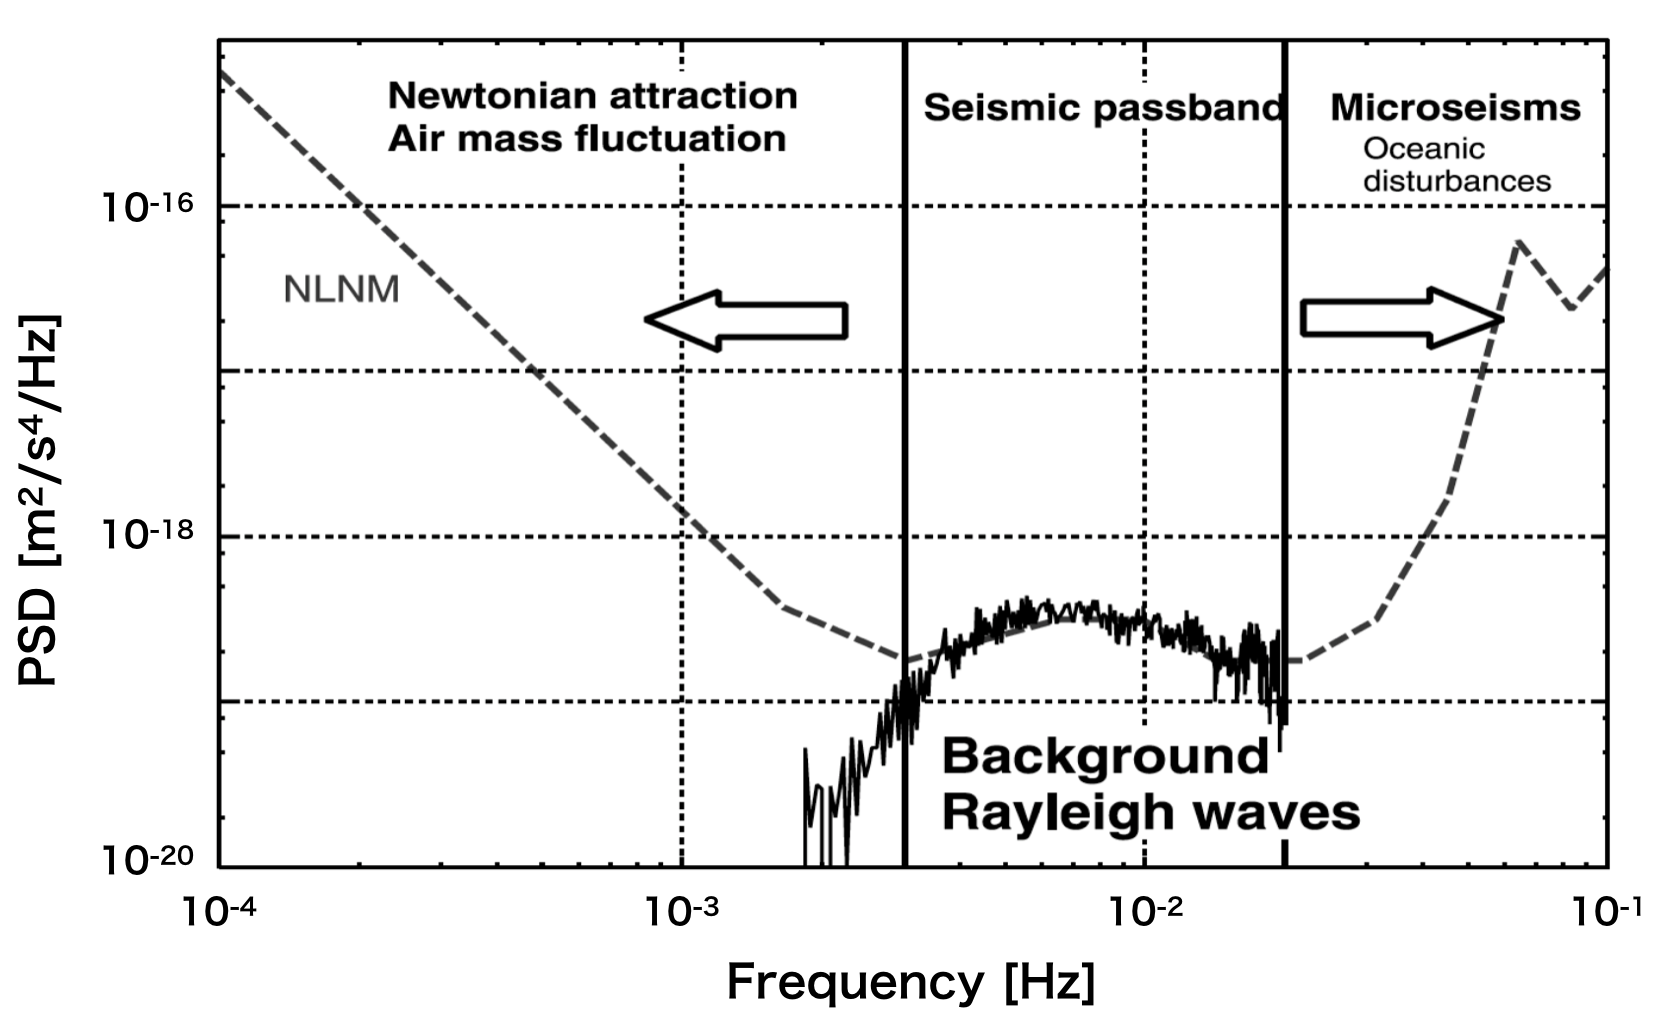
\includegraphics[width=13cm]{./img_chap3/img325.png}
    \caption{Noise contribution below $100\,\mathrm{mHz}$ \cite{nishida2002origin}. }\label{img:img325}
  \end{center} 
\end{figure}


\subsubsection{Microseisms}
Microseisms which power spectrum has peaks in $50$--$200\,\mathrm{mHz}$ are excitated by oceanic waves. These seismic waves can be categolized by the generating mechanism of these \cite{Bormann2012new}. First, the primary ocean microseisms are generated only in shallow waters in coastal regions. In this regions, the water wave enery can be converted directly into seismic energy either through vertical water pressure variations, or by the impacts of surf on the shores. There are correlation between this microseismic peak and the swell at the beaches was known starting from the data sets studied by \cite{haubrich1963comparative}. Second, the secondary ocean microseisms could be explained by the superposition of ocean waves of equal period traveling in opposite directions. Therefore, generating standing gravity waves of half the period \cite{longuet1950theory}.

The RMS amplitude spectral of both type of the microseisms are strongly depends on the low pressure on the ocean \cite{naticchioni2014microseismic}.

\subsubsection{Seismic Noise Below $20\,\mathrm{mHz}$}
Below the microseismic frequency band, the main seismic noise source is an atmospheric pressure change; Rayleigh waves excited by air fluctuation on the surface, and the deformation of the Earth's crust caused by the Newtonian attraction of air mass fluctuation \cite{sorrells1971earth,zurn1995noise}. Fig, \ref{img:img325} shows PSDs of the New Low Noise Model (NLNM) \cite{peterson1993observations} and the measured former noise \cite{nishida2002origin}. The noises caused by Rayleigh waves are consitent with the NLNM between $2\,\mathrm{Hz}$ and $30\,\mathrm{mHz}$. On the other hand, the noises caused by the Newtonian attraction are increase PSD increases rapidly with decreasing frequency below 2 mHz.

%% ここで特筆すべきは、2mHz以上のノイズはRayleigh waveで運ばれるため、地下に潜ればいくらか低減が期待されることである。実際に地表と地下のひずみ計による観測によってそれが示唆されている\cite{araya2007broadband}。

\subsubsection{Earth tides}
Below more lower frequency, the earth deformed by tidal forces due to the attraction of the Sun and the Moon in diurnal and semi-diurnal period \cite{agnew2005earth}. 

\subsubsection{Large Earthquake in the world}
Large magnitude earthquake excite the seismic wave in lower frequency \cite{aki2002quantitative,aki1967scaling}. Although the seismic noise in the observatory depends on the both fault and propagation path, here, we assume the same fault. In this situation, it is known that the measurement can be explained by model (omega-square model);
\begin{eqnarray}
  s(\omega) = \displaystyle\frac{S_0}{1+({\omega}/{\omega_0})^2}, \label{eq:eq_}
\end{eqnarray}
where $M_{\mathrm{s}}$ is the surface magnitude \cite{gutenberg1945study}, $S_0$ is a constant propotional to $M_{\mathrm{s}}$, $\omega_0$ is the corner frequency propotional to $(M_{\mathrm{s}})^{1/3}$. The spectral of Eq.(\ref{eq:eq_})with several surface magnitude are ploted in Fig.\ref{img:img328}. One can find that the large earthquakes trend to be concentrating in lower frequency.

\begin{figure}[h]
  \begin{center}   
    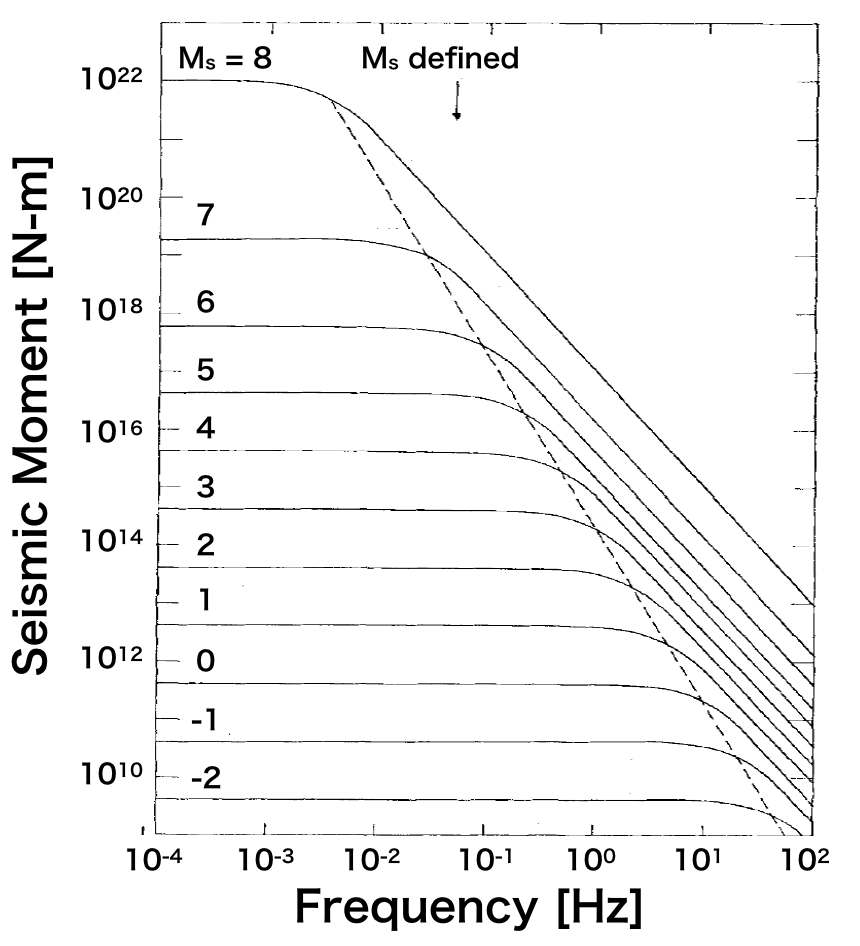
\includegraphics[width=8cm]{./img_chap3/img328.png}
    \caption{omega-square model \cite{aki1967scaling}}\label{img:img328}
  \end{center}
\end{figure}


\newpage
\section{Studies of Seismic Noise of KAGRA Mine} \label{sec:33}
\begin{figure}[h]
  \begin{center}   
    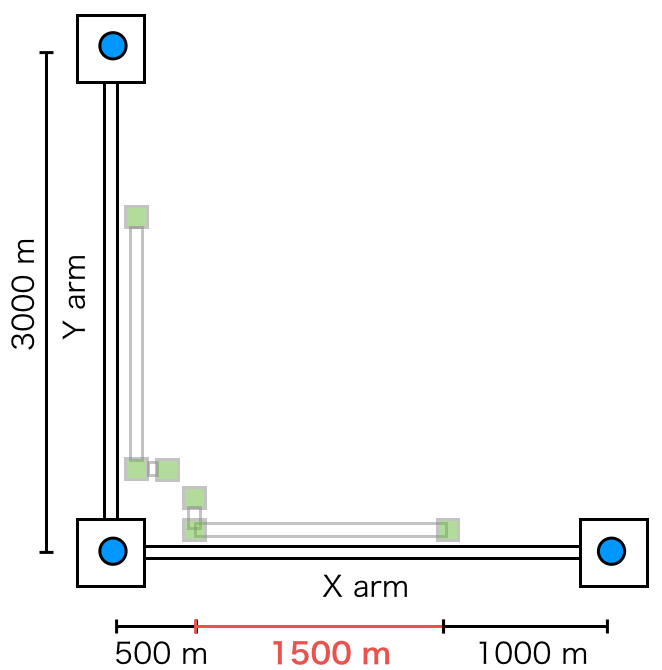
\includegraphics[width=8cm]{./img_chap3/img328a.png}
    \caption{}\label{img:img328a}
  \end{center}
\end{figure}

\subsection{Overview}
In KAGRA, we have developed the realtime seismic noise monitor using seismometers. The purpose of this system is monitor the seismic noise of the ground on which the Type-A suspensions are mounted. We installed the wide-band seismometers (Trillium 120QA) on the second floor of the corner station and each two end station. 

In this section, we have studied about the temporal and spacial characteristics of the seismic noises.

\subsection{Experimental Arrangement}\label{sec:331}
The Trillium 120-QA which is known as three-component, very broadband, and low-noise seismometer are used. These three outputs are proportional to the ground velocity of two horizontal and one vertical, respectively. 

\begin{figure}[h]
  \begin{center}   
    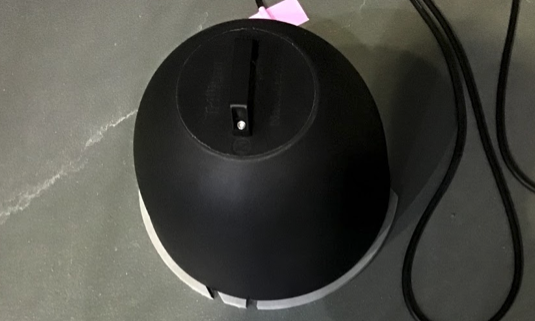
\includegraphics[width=9.0cm]{./img_chap3/img316.png}
    \caption{Trillium 120-QA installed on the second floor at X-end area, which is coverd by black thermal insulation cover}\label{img:img316}
  \end{center}
\end{figure}

The seismometer is housed in the black thermal insulation cover as shown in fig \ref{img:img316}. Thermal insulation protects two broad categories of thermal couplings that can cause unwanted noise \cite{trillium120manual}. First is the direct coupling to the sensitivity. This coupling typically increases the noise of the vertical channel as a periodic diurnal variation caused by the day-to-night temperature cycle, because the springs that suspended the inertial masses are temperature sensitive. The second is the coupling to tilt from the thermal fluctuation. Tilt converts the vertical acceleration of gravity into horizontal acceleration. This thermally induced tilt noise on the horizontal will be larger than the direct thermal coupling on the vertical channel. To be low sensitivity to both tilt and temperature, this model has a function to center the inertial mass after the initial installation.

The signals of the seismometer is recorded through the data aquisition system developed by LIGO \cite{bork2001overview}. The analog signal is converted to digital signal by the 16 bit analog-to-digital converters (ADC) with 16384 $\mathrm{Hz}$ sampling. This analog signal is amplified with 30 db so that the ADC noise does not mask this signal. 

\subsection{Data Processing}
The estimation of the amplitude spectrum densities are calculated by the average of 32 segments with 50\% overlapping. Single segment has $2^8\,\mathrm{sec}$. The FFT calculation of each segments are done after detrending the linear trend and multipling the Hanning window. 

The error bars of this spectral is calculated by chi-square distribution. For example, spectrum averaged by 32 is obey the chi-square distribution with 32 degrees of freedom. The confidence interval of $100(1-\alpha)\,\%$ with degrees of freedom $\nu$ is given by 
\begin{eqnarray}
  \frac{\nu{\hat{G}(f)}}{\chi^2(\nu,1-\frac{\alpha}{2})} \leq G(f) \leq \frac{\nu{\hat{G}(f)}}{\chi^2(\nu,\frac{\alpha}{2})},
\end{eqnarray}
where $f$ is the frequency and $\hat{G}(f)$ is estimator of spectrum. Therefore, the confidence level of 95\% is 
\begin{eqnarray}
  \nu/\chi^2(\nu,1-\frac{\alpha}{2}) \leq G(f)/\hat{G}(f) \leq \nu/\chi^2(\nu,\frac{\alpha}{2}).
\end{eqnarray}
In case that degrees of freedom is 32, the spectral point lies within 0.65 to 1.75 of the estimates.

\subsection{Study of Long-term Seismic Noise}
Long-term seismic noise is measured by a seismometer installed on the second floor of the X-end area. This area is placed 200 $\mathrm{m}$ underground from the surface of the mountain. In comparison to corner area, human activity in the end area is less because the corner area has parking lots. In comparison to the Y-end area, there is no entrance connected to other mines. Therefore, the X-end area is relatively quiet in the KAGRA mine, regarding the seismic noise induced by human activity. 

We estimated the noise spectral using the 1 year data which does not include the glitch noises such as the earthquake or circuit noise. Fig.\ref{img:img313} shows the amplitude spectrum densities (ASDs) of the horizontal and vertical components of the acceralation.

Below $40\,\mathrm{mHz}$, the horizontal noise is much larger than the vertical noise due to noise arised by temperature fluctuation, and the 10 percentile of vertical noise is close to the NLNM of Peterson. This means that the KAGRA mine is also quiet enough to measure the background seismic noise floor in this band.

From $40\,\mathrm{mHz}$ to $1\,\mathrm{Hz}$, in the microseismic noise band, the 10 percentile of both components are middle of the NHNM and NLNM. This indicates that the microseismic in KARGA is not quieter than that in inland station because KAGRA site is locate on $40\,\mathrm{km}$ far from Toyama bay. 

Above $1\,\mathrm{Hz}$, both components are close to the NLNM due to the underground environment.

\begin{figure}[p]
  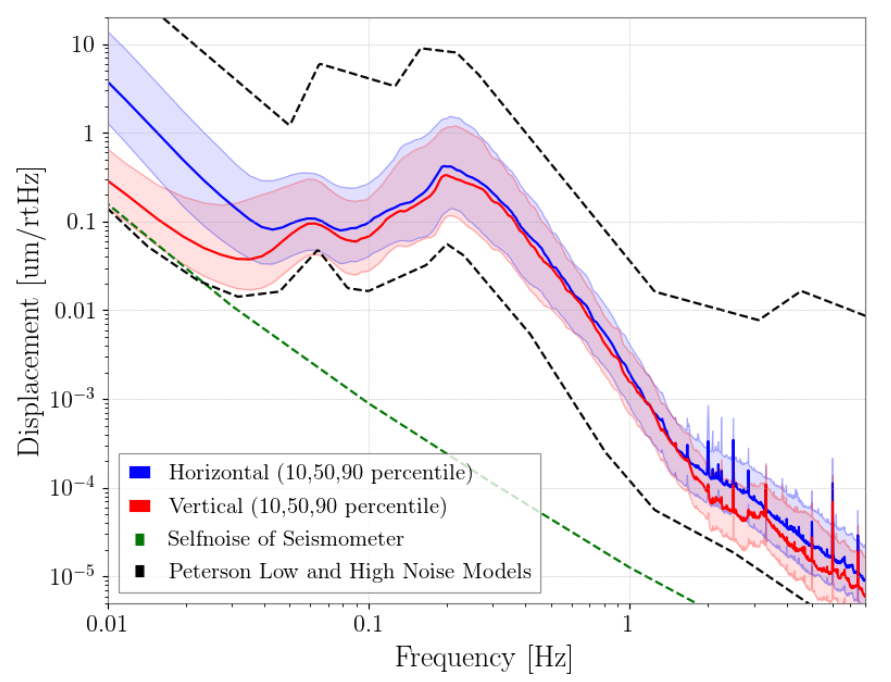
\includegraphics[width=13.0cm]{./img_chap3/img313.png}
  \caption{赤の実線は垂直成分の50パーセンタイルで、下と上に10と90パーセンタイルを示す。青の実線はX軸とY軸の二乗和から求めた並進成分であり、同様に10,50,90パーセンタイルを示す。緑点線はTrillium120 のデータシートから引用したSelfnoiseである。黒の点線はPetersonのNLNMとNHNMである。}\label{img:img313}
\end{figure}





\subsection{Study of the Differential Motion Reduction} \label{sec:332}
\cref{sec:313}でのべた差動変動の低減効果をKAGRAの地震計で計算した。



\subsubsection{CDMR in X-arm }
We calclated the CDMR, which is a ratio commom motion over differential motion of the ground given by Eq.(\ref{eq:eq23}), using two seismometers separated with $3\,\mathrm{km}$ a shown in Fig.\ref{img:img328a}. The differential and common motion of the X-arm are calculated by the X-axis of each seismometer signal, which is propotional to the ground velocity. 

The top of Fig.\ref{img:img319} shows the common and differential motion of the groung velocity. In this fifure, ASDs of the velocity of the differencial (solid line) and common motion (dashed line) are shown. The red and blue indicate the motions of X-arm and Y-arm, respectively. As a reference, black dashed line shows the selfnoise of the Trillium 120Q broadband seismometer multiplied $\sqrt{2}$. Below 0.05 Hz, the ASDs are limited by the noise mentioned in section \cref{sec:331}. 

The bottom of Fig.\ref{img:img319} shows the comparison of the CDMR calclated by these two measured motions and CDMR assumed uniform plane wave model (Bottom). The measured CDMR is given as a red and bule solid lines, which colors indicate the X-arm and Y-arm respectively. As a references, the gray line indicates the CDMR assuming the uniform plane waves model in case the phase velocity is in region from $5 - 3\,\mathrm{km/sec}$, and green dashed line is the CDMR assuming the no correlation between the each end points of the baseline. The measured CDMR is consistent with the uniform model in $0.05 - 0.5\,\mathrm{Hz}$. Below this band, the CDMR is close to the no correlation model due to the noise of the seismometers. Below and above this band, the measured CDMR is consistent with the no correlation model.

As a result, the baseline of KAGRA is well modeled with the uniform plane wave model. 

\begin{figure}[p]
    \begin{center}   
      
\includegraphics[width=13.0cm]{./img_chap3/img319.png}
      \caption{Comparison with the measured CDMR and the CDMR assumed the uniform plane waves model.}\label{img:img319}
    \end{center}
\end{figure}


%% \newpage
%% \subsubsection{Baseline length reduction}
%% We calculate the baseline length reduction given by Eq.\ref{eq:eq21} for three detectors, LISM (20 m), CLIO (100 m), KAGRA (3000 m). As mentioned in \cref{sec:141_lism}, LISM and CLIO performed a stable operation due to the short baseline. The reduction of these short-scale detectors are ploted in Fig.\ref{img:img330}. The reduction of KAGRA is plotted in Fig.\ref{img:img327}.



%% As a comparison, two types of the actuator limits are calcutated. 



%% whose baseline length is listed in table \ref{tb:31}.

%% \begin{center}
%%   \captionof{table}{Comparison of the underground GW detectors}  
%%   \begin{tabular}{lll} 
%%     \hline      
%%     Detector & Baseline length [m] & actuator limit\\ \hline \hline
%%     LISM  & 20   & \\
%%     CLIO  & 100  & \\
%%     KAGRA & 3000 & \\      
%%   \end{tabular}
%%   \label{tb:31}
%% \end{center} 


%% \begin{figure}[p]
%%   \begin{minipage}[b]{\hsize}  
%%     \begin{center}
%%       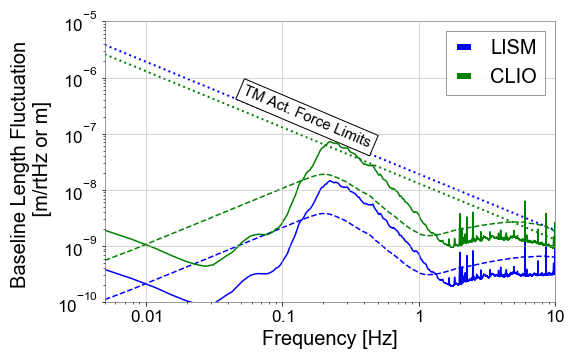
\includegraphics[width=12.5cm]{./img_chap3/img330.png}
%%       \subcaption{}\label{img:img330}
%%     \end{center}
%%   \end{minipage}\\
%%   \begin{minipage}[b]{\hsize}
%%     \begin{center}    
%%       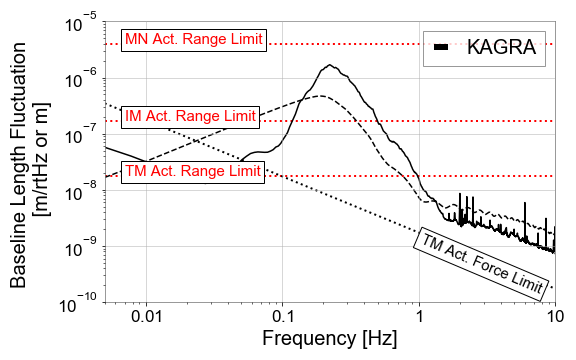
\includegraphics[width=12.5cm]{./img_chap3/img327.png}
%%       \subcaption{Comparison between the baseline length fluctuations and the displacement requirement of the underground GW detectors.}\label{img:img327}
%%     \end{center}
%%   \end{minipage}
%%   \caption{aa}  
%% \end{figure} 
%% Solid line is the baseline length fluctuation of the detectors, which is the ASD of the seismic noise (described in section \cref{sec:33}) multiplied by the function in Eq. \ref{eq:eq3} assumming the uniform plane wave model with the phase velocity of $3\,\mathrm{km/sec}$. Morever, dashed line is the accumulated RMS of the fluctuations. As a comparison, the displacement requirement of the detector, which is the linewidth of the arm cavity, is ploted.

%% \textcolor{red}{あああ}





\section{Summary of the Chapter}
